\chapter{\MakeUppercase{System Design}}

\section{System Architecture}
Simulator architecture consists of independent modules. Environment deals with time management, node generation, message generation, mobility events, neighbor finding, delivery checks, expirations, and metric computations. Routing modules deal with forwarding specific to particular protocols. Such architecture enables one to use the same environment for different routers without modifying testing conditions.

\begin{figure}[h!]
    \centering
    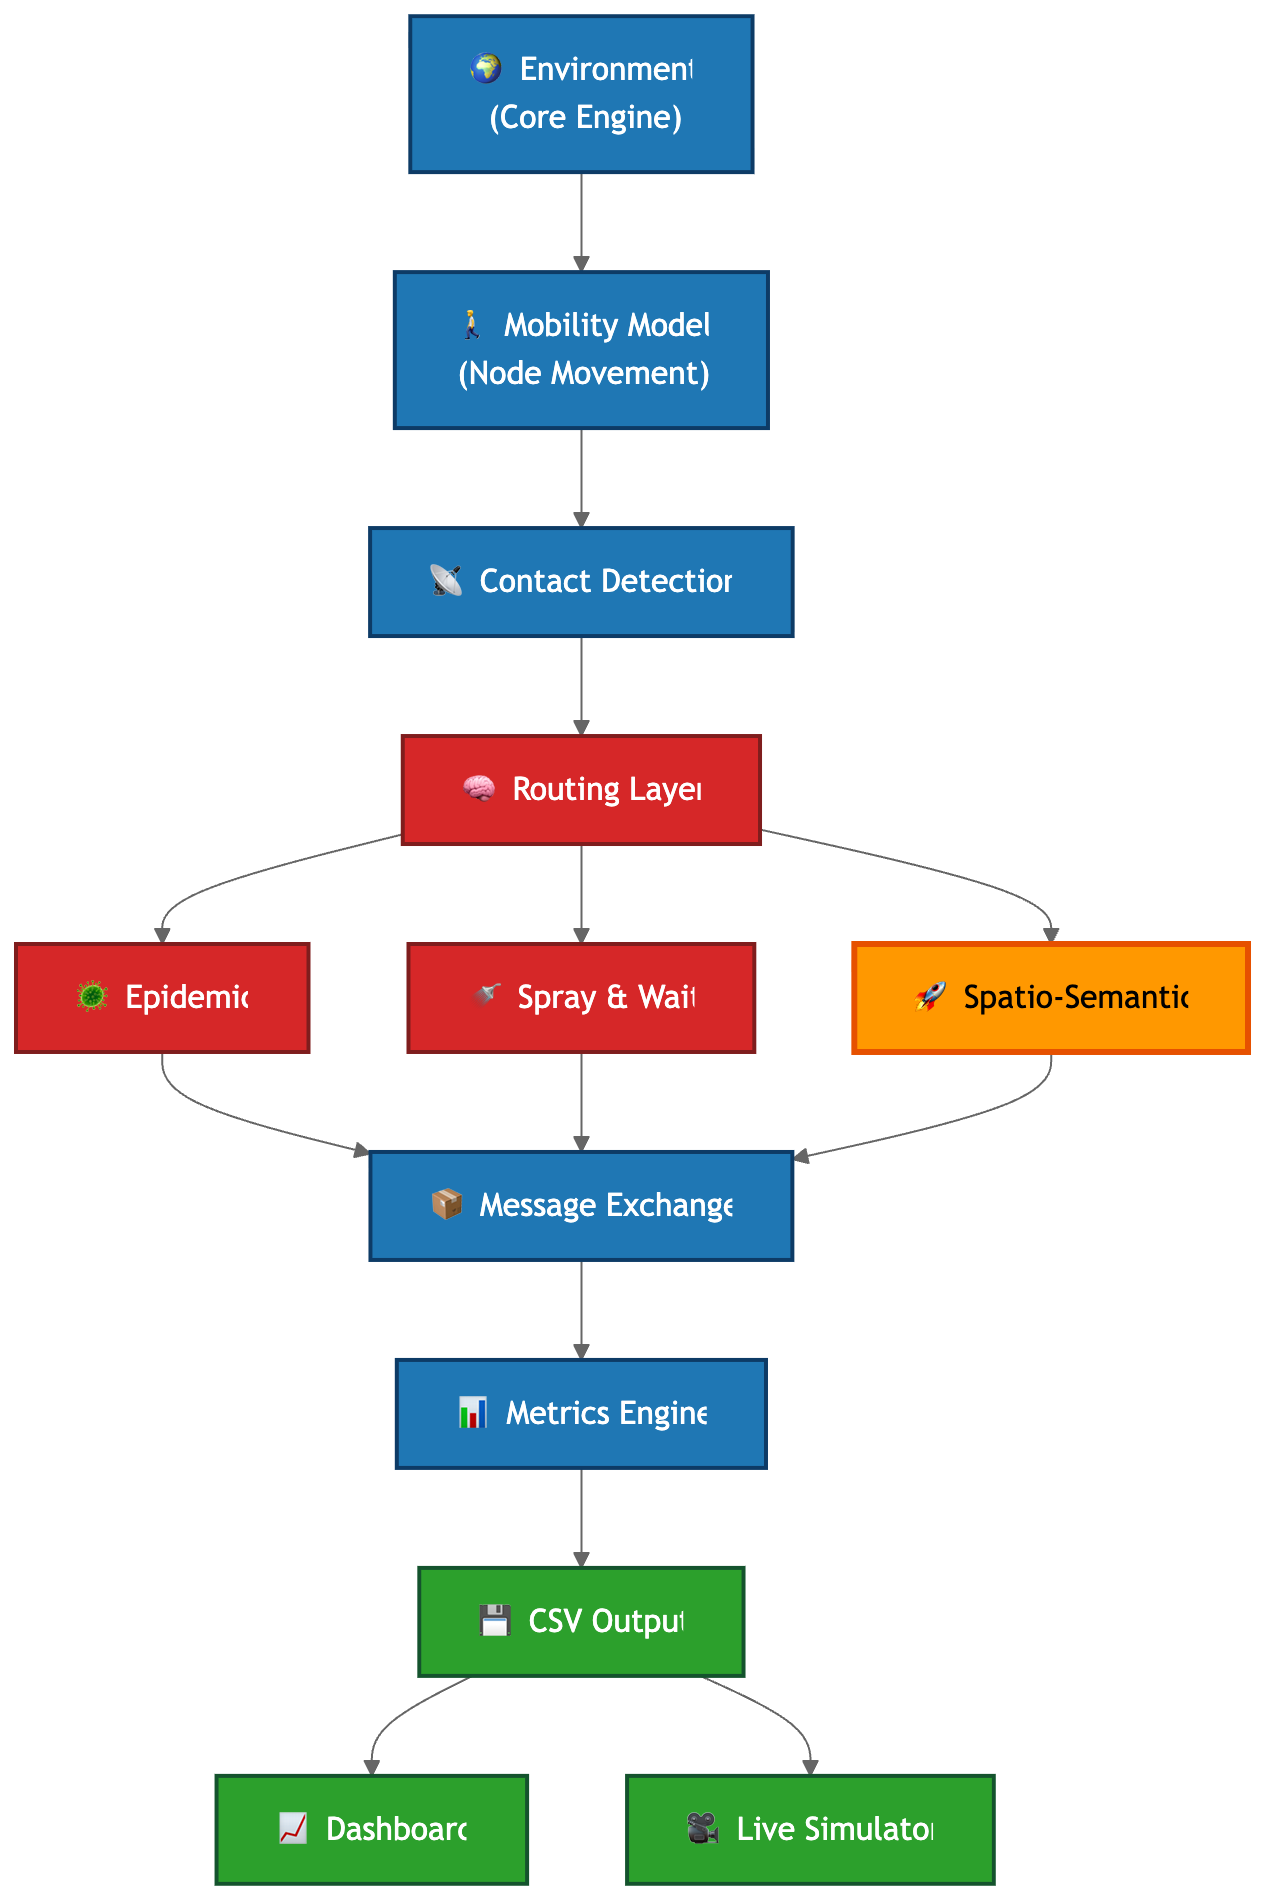
\includegraphics[width=0.65\textwidth]{images/system-arch.png}
    \caption{System architecture of the DTN routing simulator}
    \label{fig:architecture_placeholder}
\end{figure}

\section{Detailed Design}
The main execution loop performs the following sequence for each time step:

\begin{enumerate}
	\item Generates new messages according to the traffic level.
	\item Updates mobility state of every node.
	\item Detects all node pairs within transmission range.
	\item Invokes the selected router for each contact.
	\item Checks whether any message has reached its destination.
	\item Expires messages whose \ac{ttl} has been exceeded.
\end{enumerate}

Such an approach ensures that routing remains local to contacts. The router is not privy to any global foresight; rather, it makes do with the information kept within nodes and at the time of contact.

\section{Module Responsibilities and Data Flow}
Each module has an exclusive scope so that any behavior regarding routing can be examined independent of any other aspect that could complicate this process unnecessarily. It is the job of the environment to deal with the passage of time in the simulation and the enforcement of common policies like message lifetime, delivery accounting, and data aggregation. It is the node’s job to keep track of its own local state data, like mobility data, buffers, encounters, and zones.

The exchange of information among modules takes place using the same pattern in each run. The environment produces nodes and the router initialization process is carried out. Messages produced during the time interval are placed in the buffers of the sources. Mobility manipulations lead to changes in the node coordinates, and these become the basis for forming contacts at each time step. For every contact, the router module uses the local states of the two nodes, processes the encounter information, and follows routing principles. After routing activities, the environment determines if the messages have arrived at their destination points and modifies the values of the metric parameters.

\section{Proposed Spatio-Semantic Routing Design}
The Spatio-Semantic router computes a utility score for each possible carrier-destination pair. The score combines spatial proximity, direct encounter history, zone co-location, semantic role, and transitive encounter evidence. The composite utility is:

\begin{equation}
	U = 0.18P + 0.28E + 0.20Z + 0.14R + 0.20T
\end{equation}

where \ac{proximity} = normalized spatial proximity; \ac{encounter} = normalized direct encounter frequency; \ac{zone}= normalized visit frequency to the destination zone;
\ac{role} = semantic role bonus; \ac{transitive}
= two-hop encounter chain score.

\subsection{Spatial Awareness}
The simulator area is divided into a 5 by 5 grid of zones. Each node records how
frequently it visits each zone, with gradual decay over time. A carrier that often visits
the destination’s zone is considered more useful than a carrier that only happens to be
close at the current instant. This is important in \acp{dtn}, where future movement can be
more valuable than present distance.

\subsection{Semantic Awareness}
Role bonus is awarded to those nodes that are operationally useful. The drone gets the maximum role bonus due to its speed, and the fact that it can connect two distant places. Role bonus given to the responder is lesser because they are more mobile and operationally useful. Shelters get a lesser role bonus since they are a significant point especially when sending messages nearby.

\subsection{Encounter and Transitive Awareness}
Direct contact history describes how frequently the two nodes meet. This accounts for recurring meetings and consistent movement. Transitive awareness focuses on the strongest peers of the carrier and determines if the destination is in the peer’s meeting history. This concept is related to history-and-transitivity routing in \ac{prophet}, but here it is one component of a broader spatial and semantic utility function \citep{lindgren2012prophet}.

\subsection{State Aging and Adaptation}
In both encounter history and zone history, decay is applied to ensure that old events do not have an overwhelming impact on current actions. This is significant when there is a crisis since movement paths may vary due to people moving to shelters, changes in assignment for first responders, or even drones being assigned elsewhere. The node that was initially useful may no longer be valuable later.

This adaptive state design also supports fairness in relay selection. Without aging, nodes that were initially central could continue to receive forwarding preference even after their usefulness declines. By gradually reducing stale evidence, the router remains responsive to current movement and contact opportunities. The result is a more realistic approximation of how opportunistic routing should behave in a changing environment.

\section{Forwarding Policy}
The forwarding policy changes according to message priority and copy count. Critical messages are processed before non-critical messages. When many copies remain, the router behaves more aggressively and distributes multiple copies. When fewer copies remain, the router becomes more selective and forwards only when the receiver has better utility. When only one copy remains, handoff is allowed only to a clearly better carrier, with a more permissive rule for drones carrying critical messages.

\begin{algorithm}[h!]
\caption{Spatio-Semantic forwarding decision}
\begin{algorithmic}[1]
\ForAll{messages in sender buffer, ordered as critical first}
	\If{receiver already has the message or no copies remain}
		\State skip the message
	\EndIf
	\If{receiver is the destination}
		\State deliver one copy directly
	\ElsIf{message is critical and copies are above spray threshold}
		\State give a larger share of copies, especially to drones
	\ElsIf{copies are greater than one}
		\State compare receiver utility with sender utility
		\If{utility gain is sufficient}
			\State transfer a proportional number of copies
		\EndIf
	\ElsIf{one copy remains}
		\State hand off only to a clearly better carrier
	\EndIf
\EndFor
\end{algorithmic}
\end{algorithm}

\section{Buffer Management}
The proposed router reserves 35 percent of each buffer for critical messages. Non-critical messages can use only the remaining buffer capacity. If a critical message arrives when the node is full, the router attempts to evict a non-critical message, prioritizing messages with redundant remaining copies. This design directly supports the thesis goal: emergency messages should survive congestion better than routine messages.

\section{Rationale for the Hybrid Design}
The proposed design is hybrid because no single forwarding behavior is sufficient across all traffic conditions. When many copies remain, cautious forwarding wastes opportunity. When only one or two copies remain, aggressive spraying wastes resources and may move the final copy to a poorer carrier. The protocol therefore changes its behavior across the life cycle of a message. This is a deliberate design decision rather than a heuristic convenience.

The same logic applies to the combination of spatial and semantic features. Proximity alone can be misleading in \acp{dtn} because a nearby node may soon move away from the destination area. Role bonuses alone would be too coarse because not every drone or responder is equally useful at every moment. Encounter history alone would underuse static but important destinations such as shelters. The hybrid utility function addresses this by allowing different forms of partial evidence to reinforce one another.

In terms of system design, the purpose of the protocol is to enhance the quality of decisions made without adding too much complexity to the router itself. It has a simple state to maintain, an understandable scoring function, and explicit forwarding threshold values that can be adjusted. This would make it a good choice for simulation purposes, and it could easily be expanded upon in the future.

\section{Design Alternatives Considered}
An alternative option was the use of a predictor model together with encounter history and transitivity. It would be less complicated than the current one; however, it fails to consider the physical nature of the network and its carriers’ role. A geographical model could be used instead of the proposed design. Such a solution would allow considering the physical locations of all nodes; however, it will overlook the role of specific entities due to their movement capabilities and purpose in the scenario.

The design selected for use in this thesis represents a compromise between these two approaches. While maintaining the simplicity of the contact-based routing algorithm, it provides sufficient context to enhance decision making. The reason why this is crucial is that an overly simple approach would overlook the specific opportunity that exists for disasters, whereas an overly complex design might be difficult to explain and implement in a thesis paper.
